%%%%%%%%%%%%%%%%%%%%%%%%%%%%%%%%%%%%%%%%%%%%%%%%%%%%%%%%%%%%%%%%%
%%% %
%%% % weiiszablon.tex
%%% % The Faculty of Electrical and Computer Engineering
%%% % Rzeszow University Of Technology diploma thesis Template
%%% % Szablon pracy dyplomowej Wydziału Elektrotechniki 
%%% % i Informatyki PRz
%%% % June, 2015
%%%%%%%%%%%%%%%%%%%%%%%%%%%%%%%%%%%%%%%%%%%%%%%%%%%%%%%%%%%%%%%%%

\documentclass[12pt,twoside]{article}

\usepackage{weiiszablon}

\author{Krzysztof Lang}

% np. EF-123456, EN-654321, ...
\studentID{EF-148853}

\title{Implementacja wybranych algorytmów wypełniania brakujących wartości, dla strumieni dużych zbiorów danych}
\titleEN{Implemetation of selected missing value filling algorithms for large data sets}


%%% wybierz rodzaj pracy wpisując jeden z poniższych numerów: ...
% 1 = inżynierska	% BSc
% 2 = magisterska	% MSc
% 3 = doktorska		% PhD
%%% na miejsce zera w linijce poniżej
\newcommand{\rodzajPracyNo}{2}


%%% promotor
\supervisor{dr Michał Piętal}
%% przykład: dr hab. inż. Józef Nowak, prof. PRz

%%% promotor ze stopniami naukowymi po angielsku
\supervisorEN{Michał Piętal, PhD}

\abstract{Treść streszczenia po polsku}
\abstractEN{Treść streszczenia po angielsku}

\begin{document}

% strona tytułowa
\maketitle

\blankpage

% spis treści
\tableofcontents
\clearpage
\blankpage


\section{Wstęp}
\clearpage


\section{Wprowadzenie do wypełniania brakujących wartości}

\subsection{Rys historyczny}
\subsection{Na czym polega wypełnianie brakujących wartości}
\subsection{Korzyści i zagrożenia}
\subsection{Perspektywy na przyszłość}
\clearpage


\section{Omówienie narzędzi i danych}

\subsection{Python}
Do przygotowania programu wykorzystanego do przeprowadzenia badań wybrano język Python.
Jest to język wysokiego poziomu, charakteryzujący się prostą składną i wysoką przejrzystoścą kodu.
Programy nie muszą być kompilowane przed uruchomieniem, co znacznie przyśpiesza proces prototypowania i debugowania.
Oznacza to też że Python jest wolniejszy od wielu innych języków, jednak w przypadku niniejszej pracy nie ma to znaczenia.
Dostępna ogromna ilość gotowych bibliotek służących do obróbki i analizy danych znacząco uprościła przygotowanie programu.
Podczas pisania kodu trzymano się dobrych praktyk, stosowano wytyczne zawarte w PEP8.
\subsection{Visual Studio Code}
Jako środowisko programowania wybrano "Microsoft Visual Studio Code". Jest to darmowy edytor kodu obsługujący wiele języków.
Ze wzglądu na otwartość kodu, dostępne jest wiele rozszerzeń do programu, które znacznie ułatwiają tworzenie nawet skomplikowanych projektów.
W celu umożliwienia pracy nad programem z wielu urządzeń
oraz dla zachowania pełnej historii tworzenia programu wykorzystano integrację "Visual Studio Code" z repozytorium GitHub.
\subsection{Biblioteki}
\subsubsection{Pandas}

\subsubsection{NumPy}
\subsubsection{Scikit}
\subsection{Źródła danych}
\subsubsection{Użyte repozytopria danych}
Aby wyniki badań niosły ze sobą odpowiednią wartość merytoryczną, potrzebne są odpowiednie zbiory danych na których zostaną przeprowadzone testy
 W celu znalezienia odpowiednich zbiorów danych, przyjęto następujące założenia:
\begin{itemize}[label=-,labelsep=0.4cm, leftmargin=1.25cm]
    \item zbiór danych musi być wystarczająco duży,
    \item zbiór danych musi zawierać odpowiedniż ilość atrybutów aby modele decyzyjne miały
    do dyspozycji wystarczającą ilość danych uczących,
    \item atrybuty powinny zawierać różnorodne typy danych w celu przetestowania wypełniania zarówno danych
    liczbowych (całkowitych i zmiennoprzecinkowych) jak i kategorycznych,
    \item zbiór danych nie może mieć pustych wartości.
\end{itemize}
Do wyszukania odpowiednich zbiorów danych wykorzystano narzędzie "Google Dataset Search".
Z jego pomocą wybrano 2 zbiory danych z róźnych dziedzin. Po uprzedniej ich obróbce zostały wykorzystane do przeprowadzenia testów algorytów wypełniania.
\subsubsection{Adult Data Set}
Zbiór danych "Adult Data Set" zawiera dane ze spisu ludności przeprowadzonego w roku 1994 w Stanach Zjednoczonych.
Jest szeroko wykorzystywany do testowania uczenia maszynowego.
Zawiera ponad 30000 rekordów i 15 atrybutów. \cite{adult} Opis atrybutów:
\begin{itemize}[label=-,labelsep=0.4cm, leftmargin=1.25cm]
    \item age: wiek spisanej osoby, liczba całkowita,
    \item workclass: rodzaj zatrudnienia, dane kategoryczne, 8 możliwych wartości,
    \item fnlwgt: jaka proporcja populacji ma identyczny zestaw pozostałych wartości, liczba całkowita,
    \item education: osiągnięty poziom edukacji, dane kategoryczne, 16 możliwych wartości,
    \item education-num: osiągnięty poziom edukacji zakodowany jako liczba całkowita,
    \item martial-status: status matrymonialny, dane kategoryczne, 7 możliwych wartości,
    \item occupation: zawód, dane kategoryczne, 14 możliwych wartości,
    \item relationship: rola w związku, dane kategoryczne, 6 możliwych wartości,
    \item race: klasyfikacja rasowa, dane kategoryczne, 5 możliwych wartości,
    \item sex: płeć, dane kategoryczne, 2 możliwe wartości,
    \item capital-gain: zysk kapitału w zwiazku z inwestycjami, liczba całkowita,
    \item capital-gain: strata kapitału w zwiazku z inwestycjami, liczba całkowita,
    \item hours-per-week: ilość godzin pracujących w tygodniu, liczba całkowita,
    \item native-country: kraj pochodzenia, dane kategoryczne, 41 możliwych wartości,
    \item attribute: czy osoba zarabia powyżej czy poniżej 50000\$ rocznie.
\end{itemize}
Ten zbiór danych został wybrany ze względu na występowanie zarówno atrybutów liczbowych jak i kategorycznych, zadowalajacą ilość rekordów oraz atrybutów.
Ma na celu przetestowanie skuteczności działania algorytmów do wypełniania brakujących miejsc w zbiorach danych z brakami w danych o różnych typach.
Nie wymaga dodatkowej obróbki przed rozpoczęciem testów. 
\subsubsection{Stock Exchange Data}
Zbiór danych "Stock Exchange Data" zawiera informacje o cenach akcji na giełdach w różnych krajach w latach 1965-2021.
Dane zostały zebrane z "Yahoo Finance", posiadającego dane o giełdzie z wielu lat w wielu krajach. Posiada ponad 100000 rekordów i 9 atrybutów. \cite{stock} Opis atrybutów:
\begin{itemize}[label=-,labelsep=0.4cm, leftmargin=1.25cm]
    \item Index: symbol wskazujacy z jakiej giełdy pochodzą dane, dane kategoryczne, 5 możliwych wartości,
    \item Date: data obserwacji, dane kategoryczne,
    \item Open: cena akcji podczas otwarcia, liczba wymierna,
    \item High: najwyższa cena w ciągu dnia, liczba wymierna,
    \item Low: najniższa cena w ciągu dnia, liczba wymierna,
    \item Close: cena akcji w momencie zamknięcia, liczba wymierna,
    \item Adj Close: cena akcji w momencie zamknięcia skorygowana o podziały jak i dywidendy, liczba wymierna,
    \item Volume: liczba akcji będących przedmiotem obrotu w ciągu dnia sesyjnego, liczba całkowita,
    \item CloseUSD: cana akcji w momencie zamknięcia wyrażona w dolarach amerykańskich
\end{itemize}
Ten zbiór danych został wybrany ze względu na bardzo popularną kategorię danych, to jest dane finansowe.
Ma na celu przetestowanie skuteczności działania algorytmów w przypadku danych numerycznych, w szególności liczb wymiernych.
W celu lepszego przygotowania do testów zakodowano kolumnę "Data" z wykorzystaniem "label encoding", to jest zamiany danych na postać numeryczną.
Usunięto też rekordy posiadające wartość "0" w kolumnie "Volume". Ich duża ilość (ponad 30\%) mogła by negatywnie wpłynąć na uczenie modeli decyzyjnych.
W wyniku tego zmniejszono liczbę rekordów do ponad 62000, co wciąż jest ilością spełniajacą założenia dla zbiorów danych.
\clearpage


\section{Implementacja i testy algorytmu}

\subsection{Opis przygotowanego programu}
Program został napisany w języku Python, z implementacją prostego interfejsu graficznego. Został nazwany "NaN Suite".
Program miał spełniać 3 role:
\begin{enumerate}[label=\arabic*), leftmargin=1.25cm]
    \item Przygotować dane do wypełniania poprzez sztuczne utworzenie brakujacych wartości.
    \item Wypełnić brakujące wartości z wykorzystaniem wybranych algorytmów.
    \item Ocenić skuteczność wypełniania w celu porównania algorytmów.
\end{enumerate}
Poszczególne role zrealizowano jako osobne moduły. W kolejnych podrozdziałach zaprezentowane zostanie działanie programu na przykładowym pliku.
Po uruchomieniu programu pokazuje się okno służące do wyboru modułu.

\begin{figure}[ht]
	\centering
	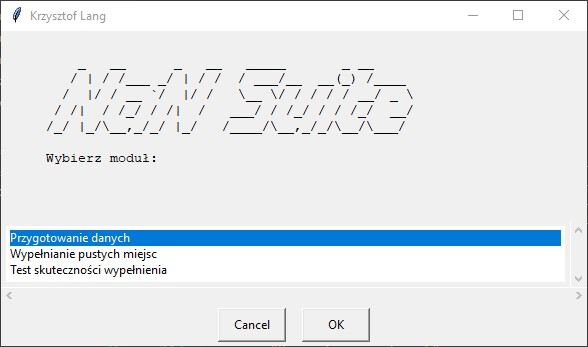
\includegraphics[width=12cm]{img/01.jpg}
	\caption{Główne okno programu, pozwalajace na wybór modułu do uruchomienia}
\label{Fig:main}
\end{figure}

\subsubsection{Tworzenie brakujących wartości}
Pierwszy moduł odpowiada z przygotowanie danych do wypełniania. Pierwszym krokiem jest wybranie pliku który ma zostać przygotowany.

\begin{figure}[ht]
	\centering
	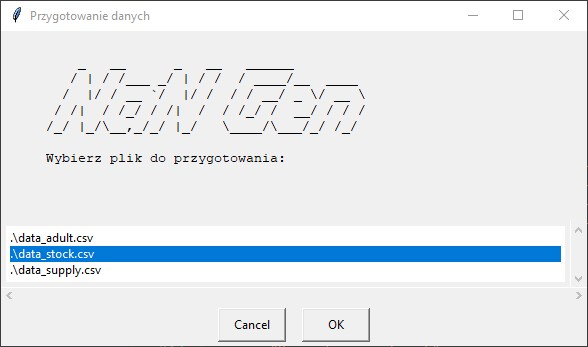
\includegraphics[width=12cm]{img/02.jpg}
	\caption{Okno wyboru pliku do przygotowania}
\label{Fig:gen_file}
\end{figure}

Następnie wybrane zostają kolumny w których maja zostać usunięte dane. Wybrać można dowolną ilość, lecz zalecane jest poniżej 50\%.

\begin{figure}[ht]
	\centering
	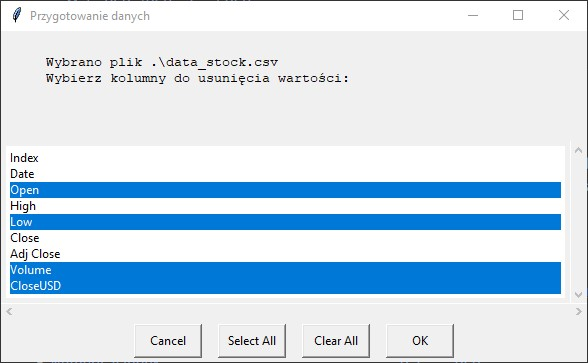
\includegraphics[width=12cm]{img/03.jpg}
	\caption{Okno wyboru kolumn}
\label{Fig:gen_col}
\end{figure}

\subsubsection{Wypełnianie brakujacych wartości}
\subsubsection{Sprawdzenie skutecznosci wypełniania}
\subsection{Opis implementacji}
\subsubsection{Alg 1}
\subsubsection{Alg 2}
\subsubsection{Alg 3}
\subsection{Napotkane problemy}
\subsection{Testy algorytmów na wybranych źródłach danych}
\clearpage


\section{Podsumowanie i wnioski końcowe}

\clearpage


\section*{Załączniki}

\addcontentsline{toc}{section}{Załączniki}

\clearpage


\addcontentsline{toc}{section}{Literatura}

\begin{thebibliography}{4}
    \bibitem{adult} archive.ics.uci.edu/ml/datasets/adult. Dostęp 26.02.2023.
    \bibitem{stock} www.kaggle.com/datasets/mattiuzc/stock-exchange-data. Dostęp 26.02.2023.
\end{thebibliography}

\clearpage


\makesummary

\end{document} 
